\documentclass{beamer}
\usepackage{tikz}
\usepackage{hyperref}
\usepackage{wasysym}
\usepackage{graphicx}
\usepackage{mathtools}
\usetheme{Singapore}
\beamertemplatenavigationsymbolsempty
\title{\\ $ $ \\ $ $ \\ The Perfect Matching Polytope}
\author{Jake Ryder Gameroff \\ Honours Research Project \\ August 7, 2024}
\date{}
\usefonttheme{serif}
\begin{document}
%{\usebackgroundtemplate{\tikz\node[opacity=0.55, inner sep=0pt] {\includegraphics[width=\paperwidth,height=\paperheight]{/Users/jakeg/Desktop/match-being-burned-alone-fl85eyvey6vse4wl.jpg}};}
\frame{\titlepage}
%! TeX root: ../mpolytope.tex

\begin{frame}
\frametitle{Agenda} \textbf{Plan for today:} 
\begin{itemize}
	\item<2-> Quick review of linear programming \& polytopes
	\item<3-> Fundamentals of matching theory
	\item<4-> The perfect matching polytope
		\begin{itemize}
			\item<5-> Bipartite \& general graphs
			\item<6-> Application to cubic graphs
		\end{itemize}
\end{itemize}
\end{frame}

\begin{frame}
\begin{center}
	\Large \textbf{Linear Programming \& Polytopes}
\end{center}
\end{frame}

\begin{frame}
\frametitle{Linear Programming}
The goal of \textbf{linear programming} is to maximize (or minimize) a linear objective function subject to a collection of linear constraints. \\
\vspace{0.3cm}
\pause
For example:
\begin{align*}
\text{maximize} \quad &z = 5x_1 + 3x_2 - 7x_3 \\
\text{subject to} \quad & x_1 + x_2 + x_3 \leq 12 \\
& 4x_1 + 5x_3 \leq 50 \\
& x_1, x_2, x_3 \geq 0
\end{align*}
\end{frame}

\begin{frame}
We can express a linear program (LP) compactly using matrices:
\pause
\begin{itemize}
	\item<2-> Goal: Find a vector \( x \) such that \( c^{T} x \) is maximized and \( x \) satisfies the constraints \( A x \leq b \) and \( x \geq 0 \).
	\item<3> (\( x, c \in \mathbb{R}^{n}  \), \( A \in \mathbb{R}^{m \times n} \), and \( b \in \mathbb{R}^{m}  \))
\end{itemize}
\end{frame}

\begin{frame}
    \frametitle{The Dual of an LP}

    Given a linear program in standard form:
    \begin{align*}
        \text{maximize} \quad & c^T x \\
        \text{subject to} \quad & Ax \leq b \\
                                & x \geq 0.
    \end{align*}
    \pause
    The dual LP is formulated as:
    \begin{align*}
        \text{minimize} \quad & b^T y \\
        \text{subject to} \quad & A^T y \geq c \\
                                & y \geq 0.
    \end{align*}
\end{frame}

\begin{frame}
\frametitle{The Dual of an LP}
The primal and dual LPs provide bounds on each other’s optimal values. If an LP has an optimum at \(x = \hat{x}  \), then its dual also has this optimum (Strong duality theorem).
\end{frame}

\begin{frame}
\frametitle{Polytopes}
A \textbf{polytope} is the convex hull of a finite collection of vectors.
\end{frame}

\begin{frame}
\frametitle{Polytopes}
\begin{figure}
        \centering
        \begin{minipage}{0.32\textwidth}
            \centering
            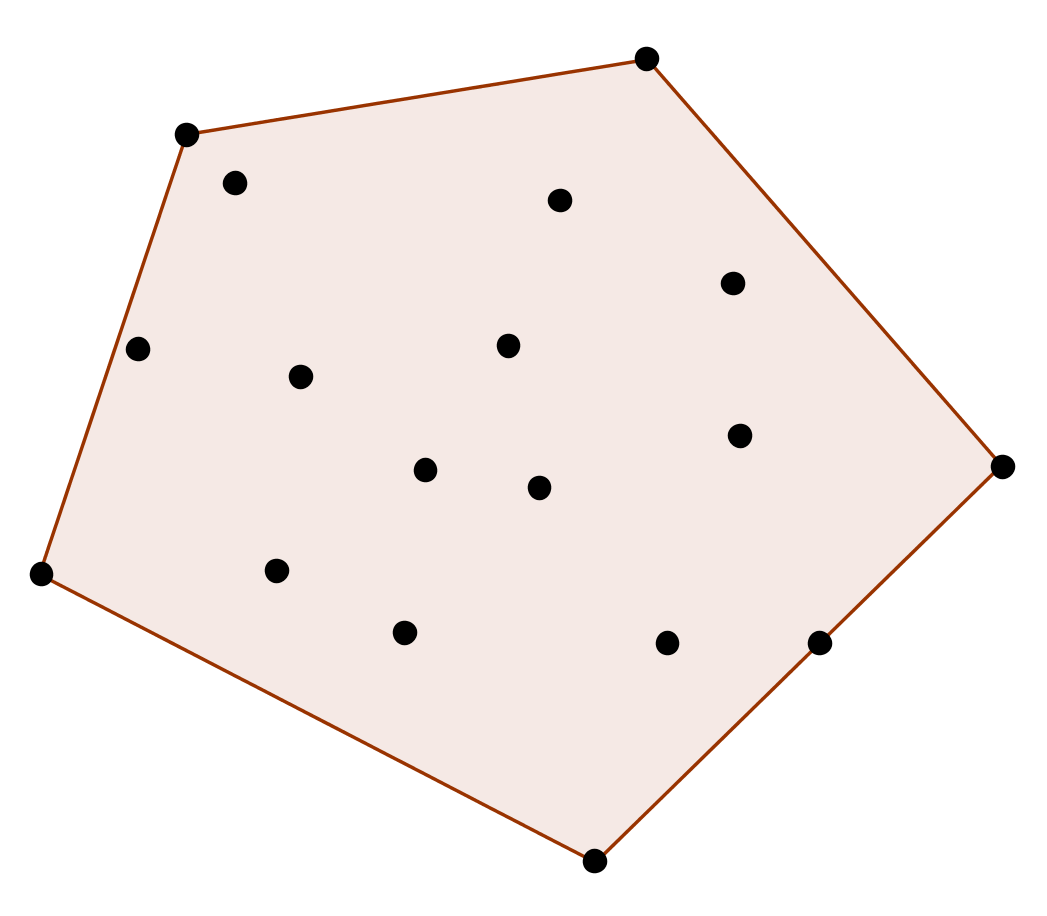
\includegraphics[width=\linewidth]{/Users/jakeg/Desktop/Matching Polytope/images/convexhull.png}
        \end{minipage}\hfill\pause
        \begin{minipage}{0.32\textwidth}
            \centering
            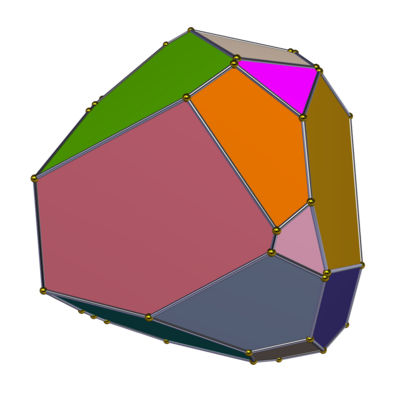
\includegraphics[width=\linewidth]{/Users/jakeg/Desktop/Matching Polytope/images/convex-polytope.png}
        \end{minipage}\hfill\pause
        \begin{minipage}{0.32\textwidth}
            \centering
            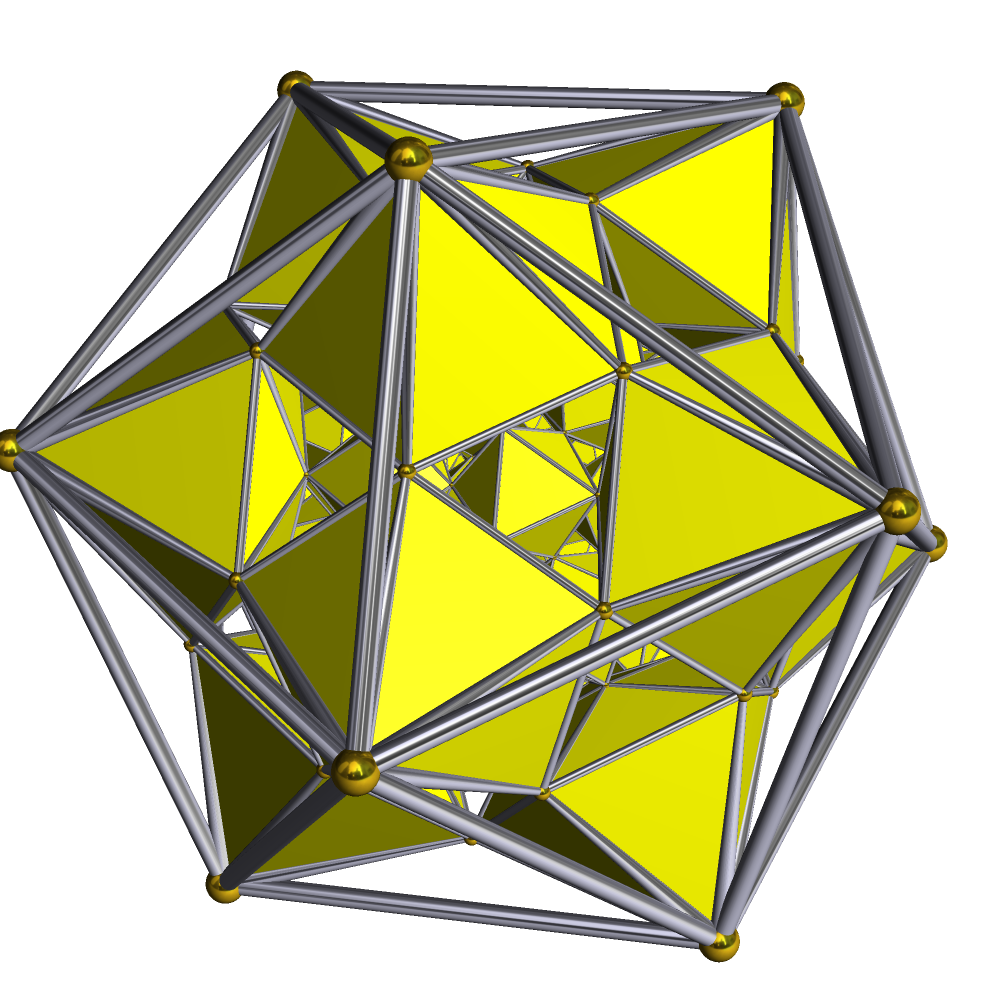
\includegraphics[width=\linewidth]{/Users/jakeg/Desktop/Matching Polytope/images/600cell.png}
        \end{minipage}
\end{figure}
\end{frame}

\begin{frame}
\begin{center}
	{\Large How are polytopes related to LP?} \\
	\vspace{0.3cm}
	\pause
	\emph{via an equivalent definition...} 
\end{center}
\end{frame}

\begin{frame}
\frametitle{Polytopes \& LP}
A vector \( \mathbf{x} \) is called a \textbf{feasible solution} if it satisfies the linear constraints of the LP, i.e. if \( A \mathbf{x} \leq \mathbf{b} \) and \( \mathbf{x} \geq \mathbf{0} \).\\
\pause
\vspace{0.3cm} The set \( P = \{ \mathbf{x} \geq \mathbf{0} : A\mathbf{x} \leq \mathbf{b} \}  \) of all feasible solutions is called a \textbf{polyhedron}. 
\begin{itemize}
	\item<3-> Bounded polyhedra are called \textbf{polytopes}.
	\item<4-> If the set of all feasible solutions to an LP is a polytope, then one of its corners is an optimum.
\end{itemize}
\end{frame}

\begin{frame}
\frametitle{The Big Picture}
We would like to solve combinatorial optimization problems using algorithms.\\
\pause
\vspace{0.3cm}
Some examples:
\pause
\begin{itemize}
	\item Finding min-weight edge or vertex covers in graphs.\pause
	\item Finding (pure, mixed, correlated) Nash equilibria in games. \pause
	\item Finding max flows and min cuts in flow networks. \pause
	\item Finding min-weight perfect matchings in graphs. \pause
\end{itemize}
\vspace{0.3cm}
If we can reduce these problems to solving linear programs, we can leverage efficient LP solvers to obtain optimal solutions.
\end{frame}

\begin{frame}
\begin{center}
\Large This talk is about the connection between linear programming, polytopes, and perfect matchings.
\end{center}
\end{frame}

\begin{frame}
\frametitle{Perfect Matchings}
A \textbf{matching} in a simple graph \( G = (V,E) \) is a subset \( M \subseteq E \) of edges such that no two edges in \( M \) share an end. \pause So every vertex \( v \in V \) is incident to \emph{at most} one edge in \( M \). \\
\pause
\vspace{0.3cm}

A matching \( M \) is \textbf{perfect} if every vertex \( v \in V \) is incident to \emph{exactly} one edge in \( M \). 
\end{frame}

\begin{frame}
\frametitle{Perfect Matchings}
A perfect matching (red edges) in the Petersen graph:
\begin{center}
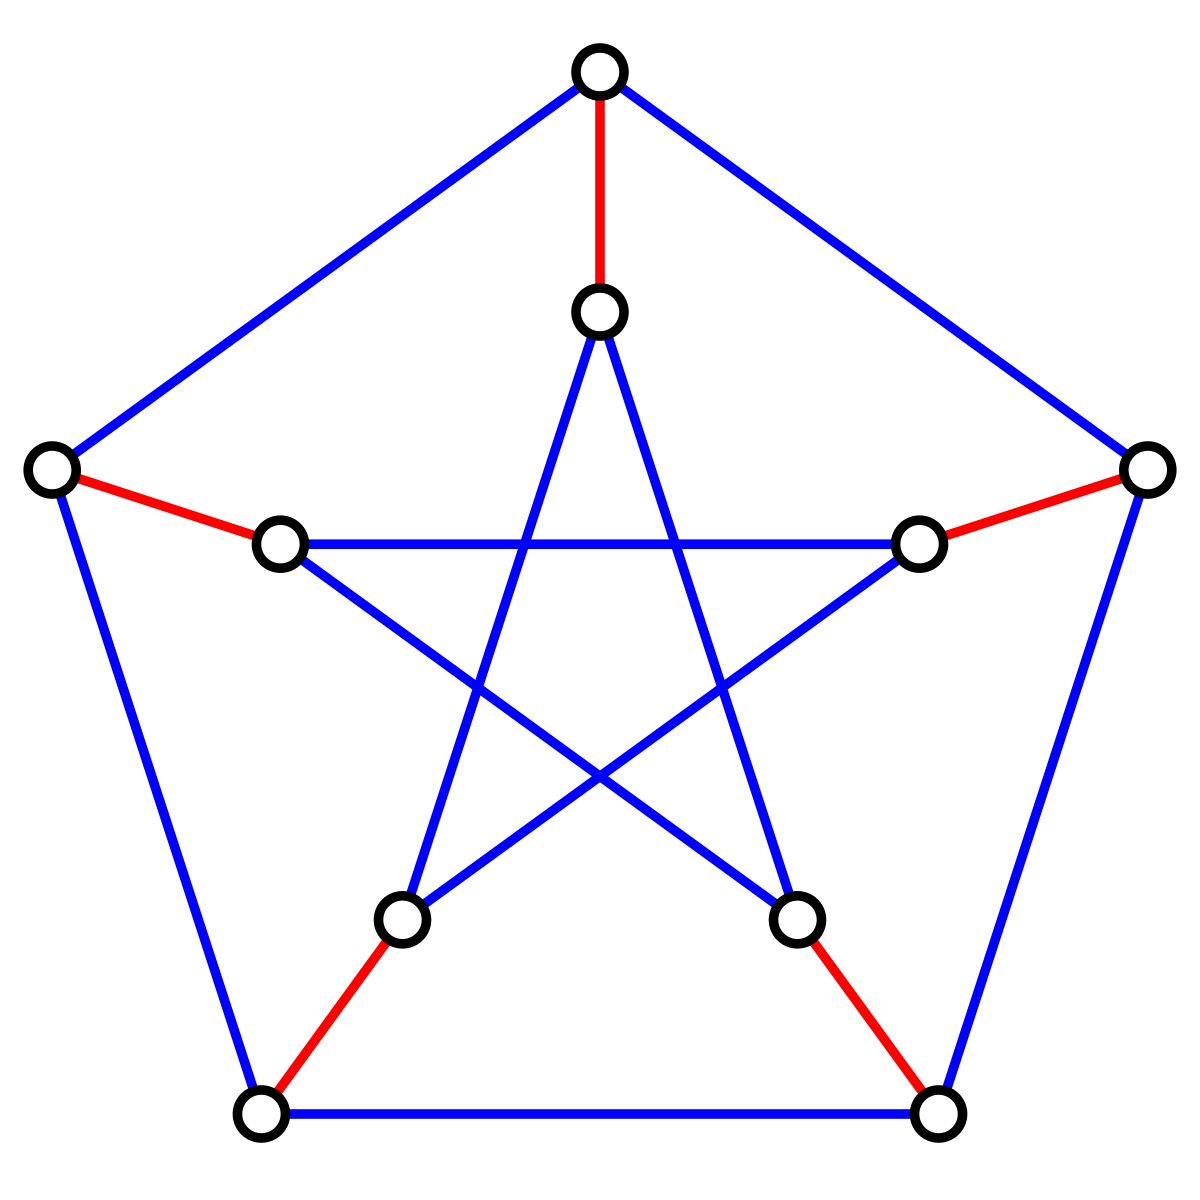
\includegraphics[scale=0.1]{/Users/jakeg/Desktop/Matching Polytope/images/peter-match.png}
\end{center}
\end{frame}

%! TeX root: ../mpolytope.tex

\begin{frame}
\begin{center}
\Large \textbf{The Perfect Matching Polytope} 
\end{center}
\end{frame}

\begin{frame}
\frametitle{Preliminaries}
Let \( G = (V,E) \). We will work in the vector space \( \mathbb{R}^{E} \coloneqq \mathbb{R}^{|E|}  \).\pause
\begin{itemize}
	\item Vectors in \( \mathbb{R}^{E}  \) have components indexed by \( E \).\pause
	\item E.g. \( x = (x(e) : e \in E) \in \mathbb{R}^{E} \). \pause
\end{itemize}
\vspace{0.3cm}
As such, each component of a vector in \( \mathbb{R}^{E}  \) contains information about an edge \( e \in E \). \pause
\begin{itemize}
	\item E.g. If \( F \subseteq E \), define \( \chi_{F} \in \mathbb{R}^{E}  \) by \( \chi_{F}(e) = 1  \) if \( e \in M \) and \( \chi_{F} (e) = 0 \) otherwise.
\end{itemize}
\vspace{0.3cm}
\end{frame}

\begin{frame}
\frametitle{Preliminaries}
We must cover one final preliminary:\pause \\
\vspace{0.3cm}
Given \( x \in \mathbb{R}^{E}  \) and \( F \subseteq E \), define \pause \[ x(F) \coloneqq x \cdot \chi_{F} = \sum_{e \in F}^{} x(e) .  \]
\end{frame}

\begin{frame}
\frametitle{The Perfect Matching Polytope}
Let \( \mathcal{M}_{G}  \) denote the collection of perfect matchings of \( G \). Then, we define the \textbf{perfect matching polytope} \( \mathcal{P} \mathcal{M}  (G) \) of \( G \) by \pause \[ \mathcal{P} \mathcal{M} (G) \coloneqq \operatorname{conv} (\{ \chi_{M} \in \mathbb{R}^{E} : M \in \mathcal{M} _{G}  \} ), \] \pause where \( \operatorname{conv} (A) \) is the smallest convex set containing \( A \subseteq \mathbb{R}^{E}  \).
\end{frame}

\begin{frame}
\frametitle{The Perfect Matching Polytope}
The set \( \mathcal{P} \mathcal{M} (G) = \operatorname{conv} (\{ \chi_{M} \in \mathbb{R}^{E} : M \in \mathcal{M} _{G}  \} ) \) doesn't seem to help us investigate the perfect matchings in \( G \).
\begin{itemize}
	\item<2-> By definition, \( \mathcal{P} \mathcal{M} (G) \) is a polytope, so it would be really nice if we could \emph{find a linear program} whose optimum occurs at one of its corners. 
	\item<3> Let's do that now!
\end{itemize}
\end{frame}

\begin{frame}
\frametitle{The Perfect Matching Polytope}
\textbf{Observation 1:} \emph{If \( x \in \mathcal{P} \mathcal{M} (G) \), then \( x(e) \geq 0 \) for every \( e \in E \).} \pause
\begin{proof}
	We may write \( x \) as a convex combination of characteristic vectors of perfect matchings in \( G \): \[ x = \lambda_1 \chi_{M_1} + \lambda_2 \chi_{M_2} + \cdots + \lambda_{n} \chi_{M_{n} } . \] \pause Since \( \lambda_{j} \in [0, 1] \) and \( \chi_{M_{j} } \geq 0 \) for each \( j \in [n] \), it follows that \( x \) has non-negative components.
\end{proof}
\end{frame}

\begin{frame}
\frametitle{The Perfect Matching Polytope}
\textbf{Observation 2:} \emph{If \( x \in \mathcal{P} \mathcal{M} (G) \), then \( x(\delta (v)) = 1 \) for all \( v \in V \).}\\
\pause (\emph{note: \( \delta (X) \) is the set edges with exactly one end in \( X \)})\pause

\begin{proof}
Again, write \( x = \sum_{j=1}^{n} \lambda_{j} \chi_{M_{j} }  \) as a convex combination. Then \pause
\begin{align*}
	x(\delta (v)) &= \sum_{e \in \delta (v)}^{} x(e) = \sum_{e \in \delta (v)}^{} \sum_{j=1}^{n} \lambda_{j} \chi_{M_{j} } (e) \\
		      &= \sum_{j=1}^{n} \sum_{e \in \delta (v)}^{} \lambda_{j} \chi_{M_{j} } (e) = \sum_{j=1}^{n} \lambda_{j} = 1,
\end{align*}
since each \( M_{j}  \) is a perfect matching.
\end{proof}
\end{frame}

\begin{frame}
\frametitle{The Perfect Matching Polytope}
\textbf{Observation 1:} \emph{If \( x \in \mathcal{P} \mathcal{M} (G) \), then \( x(e) \geq 0 \) for every \( e \in E \).} \\
\vspace{0.1cm}
\textbf{Observation 2:} \emph{If \( x \in \mathcal{P} \mathcal{M} (G) \), then \( x(\delta (v)) = 1 \) for all \( v \in V \).}\\
\vspace{0.5cm}
Observations 1 and 2 can be written compactly as the following: \pause \\
\vspace{0.1cm}
\textbf{Observtion 3:} \emph{If \( x \in \mathcal{P} \mathcal{M} (G) \), then \( x \geq 0 \) and \( Ax = 1 \), where \( A = (a_{ve})_{v \in V, e \in E}  \) is the incidence matrix of \( G \).}
\begin{itemize}
	\item<3> \emph{This is really starting to look like a linear program...} 
\end{itemize}
\end{frame}

\begin{frame}
\frametitle{The Fractional Perfect Matching Polytope}
\textbf{Observtion 3:} \emph{If \( x \in \mathcal{P} \mathcal{M} (G) \), then \( x \geq 0 \) and \( Ax = 1 \), where \( A = (a_{ve})_{v \in V, e \in E}  \) is the incidence matrix of \( G \).}\\
\vspace{0.3cm}
Define the \textbf{fractional perfect matching polytope} \( \mathcal{F} \mathcal{P}\mathcal{M} (G)  \) of a graph \( G \) by \pause \[ \mathcal{FPM}(G) \coloneqq \{ x \in \mathbb{R}^{E} : x \geq 0 \mbox{ and } Ax = 1 \}.   \] \pause Then, it follows from observation 3 that \( \mathcal{PM} (G) \subseteq \mathcal{FPM} (G) \).
\begin{itemize}
	\item<2> \emph{This raises a natural question...} 
	
\end{itemize}
\end{frame}

\begin{frame}
\begin{center}
\Large Are there any graphs \( G \) with \( \mathcal{PM} (G) = \mathcal{FPM} (G) \)?
\end{center}
\end{frame}

\begin{frame}
\begin{center}
	\Large Yes!
\end{center}
\end{frame}

\begin{frame}
\begin{center}
	\Large If \( G \) is \textbf{\alert{bipartite}}, then \( \mathcal{PM} (G) = \mathcal{FPM} (G) \).
\end{center}
\end{frame}

\begin{frame}
\textbf{Lemma 1.} \emph{Let \( A \) be the incidence matrix of a bipartite graph \( G \). Then \( A \) is totally unimodular; that is, every square submatrix \( B \) of \( A \) satisfies \( \det B \in \{ 0, \pm 1 \}  \).}\pause
\begin{proof}
Let \( B \) be an \( m \times m \) submatrix of \( A \). The proof is by induction on \( m \). If \( m = 1 \) then clearly \( \det B \in \{ 0,1 \}  \), so fix \( m \geq 2 \).
\begin{itemize}
	\item<3-> If \( B \) has a column with only zeros, then \( \det B = 0 \).
	\item<4-> If a column has exactly one non-zero entry, then we may cofactor-expand along this column and use the IH to obtain \( \det B \in \{ 0, \pm 1 \}  \).
	\item<5-> Otherwise, every column of \( B \) has exactly two non-zero entries. Since any two non-zero entries from the same column are in different partite sets, the sum of all rows pertaining to vertices from one partite set equals the sum of all rows from the other. So \( \det B = 0 \) since its rows are linearly dependent.
\end{itemize}
\end{proof}
\end{frame}

\begin{frame}
	\textbf{Lemma 2.} \emph{If \( A \) is totally unimodular and \( b \) is a vector with integer components, then all corners of \( P = \{ x \geq 0 : Ax \leq b \}  \) have integer components.}\pause
\begin{proof}
	The proof is long and somewhat off-topic. Given the time constraint, see week 8 from {\color{blue!80}{\href{https://www.math.uvic.ca/~noelj/MA252.html}{this webpage}}} for a careful and detailed consideration.
\end{proof}
\end{frame}

\begin{frame}
\textbf{Lemma 3.} \emph{If \( x \in \mathcal{FPM} (G) \) is integral, then \( x \in \mathcal{PM} (G) \).}\pause
\begin{proof}
We know that \( x(e) \geq 0 \) for each \( e \in E \) and \( \sum_{e \in \delta (v)}^{} x(e) = 1 \) for each \( v \in V \). \pause Since \( x \) is integral (i.e. has integer components), there is exactly one edge \( e \in \delta (v) \) with \( x(e) = 1 \). \pause Since this holds for each \( v \in V \), \( x \) is a characterstic vector of a perfect matching in \( G \). \pause So \( x \in \mathcal{PM} (G) \).
\end{proof}
\end{frame}

\begin{frame}
	\frametitle{The Bipartite Case}
	\textbf{Theorem.} \emph{If \( G \) is a bipartite graph, then \( \mathcal{PM} (G) = \mathcal{FPM} (G) \).}\pause
\begin{proof}
We have already seen that \( \mathcal{PM} (G) \subseteq \mathcal{FPM} (G) \). \pause From Lemma 1, the incidence matrix \( A \) of \( G \) is totally unimodular; \pause and so Lemma 2 implies that every corner of \( \mathcal{FPM} (G) \) is integral. \pause Then, Lemma 3 implies that all corners of \( \mathcal{FPM} (G) \) are in \( \mathcal{PM} (G) \). \pause By the convexity of \( \mathcal{PM} (G) \), we conclude that \( \mathcal{FPM} (G) \subseteq \mathcal{PM} (G) \).
\end{proof}
\end{frame}

\begin{frame}
	\frametitle{The Bipartite Case}
We can define the \textbf{matching polytope} of \( G \) analagously: \[ \mathcal{M} (G) \coloneqq \operatorname{conv} (\{ \chi_{M} : M \mbox{ is a matching in } G \} . \] \pause We can also define its fractional matching polytope: \[ \mathcal{FM} (G) \coloneqq \{ x \in \mathbb{R}^{E} : x \geq 0 \mbox{ and } Ax \leq 1 \}. \]
\pause We have \( Ax \leq 1 \) (rather than \( Ax = 1 \)) because every vertex is incident to \emph{at most} 1 edge in a matching.
\begin{itemize}
	\item<2> By the exact same reasoning as before, \( \mathcal{M} (G) = \mathcal{FM} (G) \) whenever \( G \) is bipartite.
	
\end{itemize}
\end{frame}

\begin{frame}
\begin{center}
\Large At this point, you're probably thinking...
\end{center}
\end{frame}

\begin{frame}
\begin{center}
	\Large \emph{``Who cares? When am I ever gonna use this?"}
\end{center}
\end{frame}

\begin{frame}
\begin{center}
\Large Well...
\end{center}
\end{frame}

\begin{frame}
\begin{center}
	\Large We can use this to prove \alert{\textbf{K\"onig's Theorem}}! :)
\end{center}
\end{frame}

\begin{frame}{K\"onig's Theorem}
Let \( G = (V,E) \). Then, we define\pause
\begin{itemize}
	\item \( \nu (G) \coloneqq  \) max size of a matching in \( G \).\pause
	\item \( \tau (G) \coloneqq \) min size of a vertex cover in \( G \).\pause
\end{itemize}
\vspace{0.3cm}
Note that \( \nu (G) \leq \tau (G) \) for every graph \( G \). \pause Indeed, given a minimal vertex cover $X$ and any matching $M$, each edge in $M$ has an end in $X$. Since no two edges in $M$ share an end, $|M| \leq |X|$. \pause Consequently, $\nu (G) \leq \tau (G)$.
\end{frame}

\begin{frame}
\textbf{K\"onig's Theorem.} The quantities \( \nu (G) = \tau (G) \) for every bipartite graph \( G \).\pause
\begin{proof}\renewcommand{\qedsymbol}{}
	From the previous theorem (and Lemmas 1-3), one of the corners of \[ \mathcal{M} (G) = \mathcal{FM} (G) = \{ x \in \mathbb{R}^{E} : x \geq 0 \mbox{ and } Ax \leq 1 \} \] gives \( \nu (G) \) as an optimum to the following (integral) LP:\pause
\begin{align*}
\text{maximize} \quad &z(x) = \sum_{e \in E}^{} x(e) \\
\text{subject to} \quad & \sum_{e \in \delta (v)}^{} x(e)  \leq 1, \ \forall v \in V \\
& x(e) \geq 0, \ \forall e \in E.
\end{align*}
(\emph{proof continues on next slide.})
\end{proof}
\end{frame}

\begin{frame}
Using a bit of algebra, one can check that the dual of the LP on the previous slide is: \pause
\begin{align*}
\text{minimize} \quad & \sum_{v \in V}^{} y(v)  \\
\text{subject to} \quad & y(u) + y(v) \geq 1 , \ \forall uv \in E \\
& y(v) \geq 0, \ \forall v \in V.
\end{align*}
\pause From the strong duality theorem, it follows that the dual has optimum value \( \nu (G) \). \pause But notice that by construction, the dual LP computes \( \tau (G) \), so \( \nu (G) = \tau (G) \).\pause \\
\vspace{0.4cm}
(Remark: the dual LP is integral. Indeed, the transpose of a totally unimodular matrix is totally unimodular, so Lemma 2 asserts the claim.) \qed
\end{frame}

\begin{frame}{The General Case}
\textbf{Remark.} There are graphs with \(\mathcal{FPM} (G) \not\subseteq \mathcal{PM} (G) \). \pause
\begin{proof}
Consider any odd cycle \( C = (V,E) \). Define the vector \( c \in \mathbb{R}^{E}  \) given by \( c(e) = 1/2 \) for each \( e \in E \). \pause Then \( c \geq 0 \) and \[ c(\delta (v)) = \sum_{e \in \delta (v)}^{} c(e) = 1/2 + 1/2 = 1,  \] since each vertex in \( C \) has exactly two neighbours. \pause So \( c \in \mathcal{FPM} (C) \). But \( c \notin \mathcal{PM} (C) \), since \( \mathcal{PM} (C) = \emptyset   \).
\end{proof}
\end{frame}

%! TeX root: ../mpolytope.tex

\begin{frame}
\begin{center}
\Large Can we extend this theory to \emph{general} graphs?
\end{center}
\end{frame}

\begin{frame}{The General Case}
	\textbf{Edmonds' Theorem.} \emph{For any graph \( G \), the polytope \( \mathcal{PM} (G) \) is precisely the set of vectors \( x \in \mathbb{R}^{E}  \) satisfying:} \pause
	\begin{enumerate}
		\item \( x \geq 0 \);\pause
		\item \( x (\delta (v)) = \sum_{e \in \delta (v)}^{} x(e) = 1  \), for each \( v \in V \); \pause
		\item \( x(\delta (X)) = \sum_{e \in \delta (X)}^{} x(e) \geq 1 \), for each odd subset \( X \subseteq V \). \pause
	\end{enumerate}
\begin{proof}
Please see Theorem 5 {\color{blue!80}{\href{https://www.math.mcgill.ca/snorin/papers/lecture2.pdf}{here}}}.
\end{proof}
\end{frame}

\begin{frame}
\begin{center}
	\Large \textbf{Application: Perfect matchings in cubic (3-regular) graphs}
\end{center}
\end{frame}

\begin{frame}
\vspace{0.3cm}
\textbf{Theorem.} \emph{Every cubic bridgeless graph has a perfect matching.} \pause
\begin{proof}
It suffices to prove that its perfect matching polytope \( \mathcal{PM}(G) \) is non-empty. \pause Put \( x = (1/3 : e \in E). \) \pause Then \( x \geq 0 \), and since \( G \) is cubic, \( x(\delta (v)) = 3 \cdot 1/3 = 1. \) \pause Finally, fix an odd subset \( X \subseteq V \) and let \( \ell = |\delta (X)| \) be the number of edges leaving \( X \). \pause Then \[3|X| = \sum_{v \in X}^{} \deg v = 2 |E(X)| + \ell. \] \pause Now observe that \( 3|X| \) is odd and \( 2|E(X)| \) is even, so \( \ell \) is odd. \pause Further, \( \ell > 1 \) since \( G \) is bridgeless, and so \( \ell \geq 3 \). \pause Hence \[ x(\delta (X)) = \sum_{e \in \delta (X)}^{} x(e) = \ell / 3 \geq 1.   \] \pause

By Edmonds' theorem, \(x = (\frac{1}{3} , \frac{1}{3} , \hdots ,\frac{1}{3} ) \in  \mathcal{PM} (G) \neq \emptyset  \).
\end{proof}
\end{frame}

\begin{frame}
\begin{center}
\Large In fact, every \( d \)-regular, \( (d-1) \)-edge-connected graph has a perfect matching.
\end{center}
\end{frame}

\begin{frame}
\begin{tikzpicture}[remember picture, overlay]
        \node [opacity=0.2] at (current page.center) {
            \includegraphics[scale=0.28]{/Users/jakeg/Desktop/Matching Polytope/images/matches.jpg}
        };
\end{tikzpicture}
\begin{center}
	\vspace{2.5cm}
	{\huge \textbf{Thanks for listening!} $\smiley$} \\
	\Large Let me know if you have any questions! \pause
\end{center}
\vspace{1.8cm}
References: We followed Lov\'asz and Plummers' book, ``Matching Theory" (1985), and used information from the notes linked {\color{blue!80}{\href{https://www.math.uvic.ca/~noelj/MA252.html}{here}}} (week 9) and {\color{blue!80}{\href{https://www.math.mcgill.ca/snorin/papers/lecture2.pdf}{here}}}.
\end{frame}

\end{document}
